%%%%%%%%%%%%%%%%%%%%%%%%%%%%%%%%%%%%%%%%%%%%%%%%%%%%%%%%
% Exemplo 06-05: newtheorem: criando ambientes de teoremas
% ultima atualizacao: 05/02/2018 por Sadao Massago
% http:/www.dm.ufscar.br/~sadao
%----------------------------------------------------
% EXEMPLO não finalizado
% talvez utilizar o AMS

\documentclass[12pt,a4paper]{article}

% T1 não é aceito no PCTeX 4.0 ou anterior.
% Neste caso, comente
\usepackage[T1]{fontenc} % codificação da fonte em 8-bits
\usepackage[utf8]{inputenc} % acentuação direta
\usepackage[brazil]{babel} % em portugues brasileiro
\usepackage{amsthm}
\usepackage{graphicx}
% \usepackage{theorem} % para configurar o teorema
\usepackage{amsthm} % para configurar o teorema (do AMS)
%\usepackage{movie15}
% \theoremstyle{plain} % o padrao. Ja esta com este estilo




\begin{document}




\begin{figure}[!htp]
\begin{center}

\includegraphics[width=10cm]{1}
\end{center}
\end{figure}

\begin{figure}
\begin{center}

\includegraphics[width=10cm]{2}
\end{center}
\end{figure}

\begin{figure}
\begin{center}
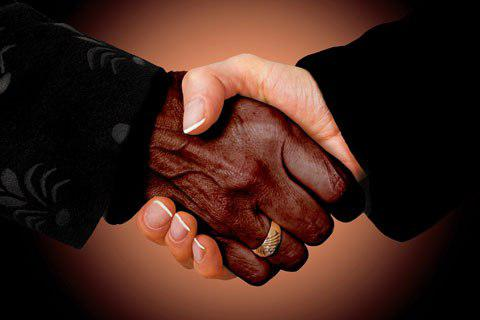
\includegraphics[width=10cm]{3}
\end{center}
\end{figure}

\begin{figure}
\begin{center}
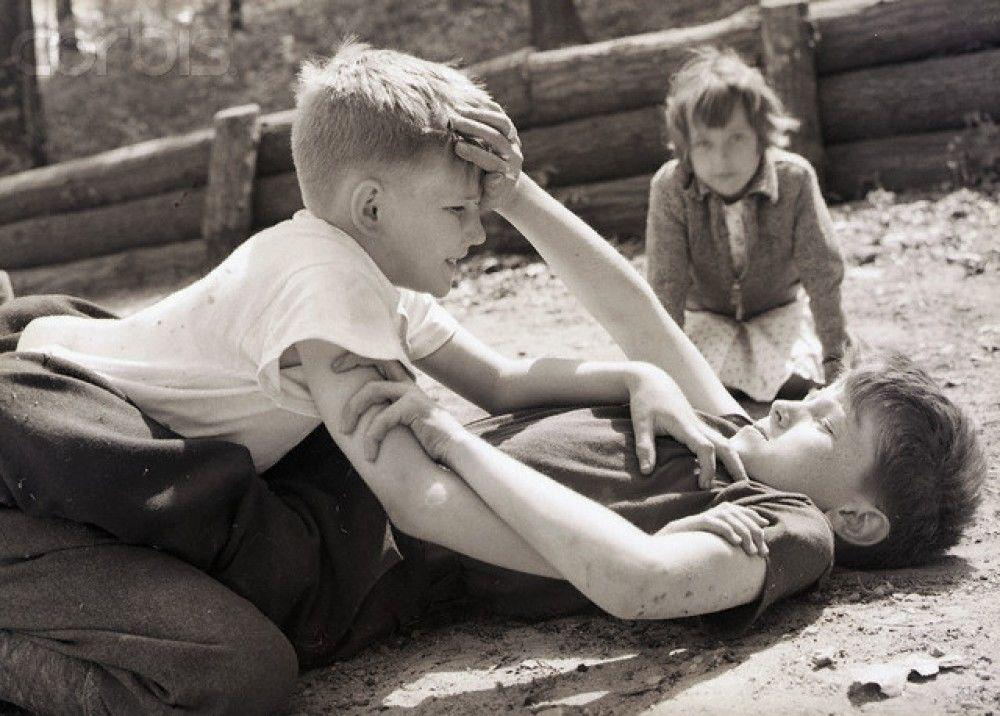
\includegraphics[width=10cm]{4}
\end{center}
\end{figure}

\begin{figure}
\begin{center}
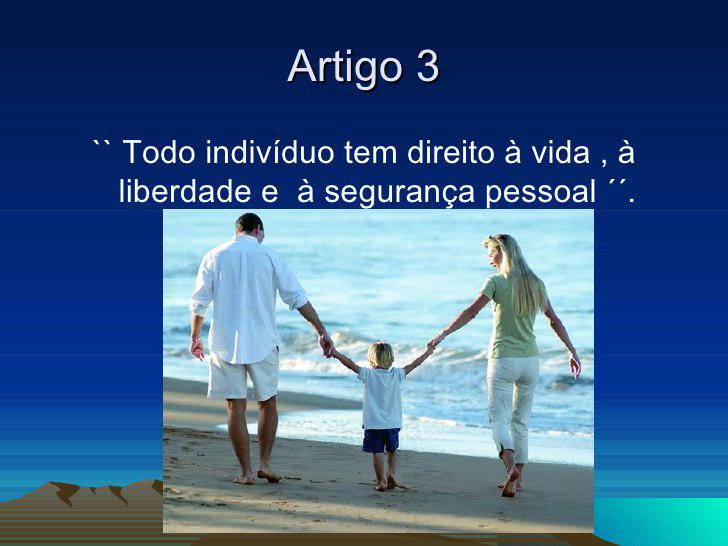
\includegraphics[width=10cm]{5}
\end{center}
\end{figure}

\begin{figure}
\begin{center}
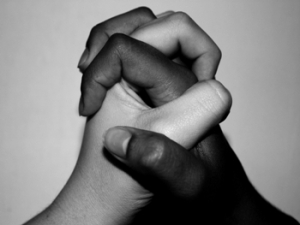
\includegraphics[width=10cm]{6}
\end{center}
\end{figure}



\end{document} % final do documento
